\documentclass[11pt,a4paper,oneside]{article}
\usepackage{color}
\usepackage[utf8]{inputenc} % Включаем поддержку UTF8  
\usepackage[russian]{babel}  % Включаем пакет для поддержки русского языка  
\usepackage{graphicx}
\usepackage{enumitem}

\graphicspath{ {./images/} }
\DeclareGraphicsExtensions{.png,.pdf,.jpeg,.jpg}

\DeclareUnicodeCharacter{F7}{$\div$}
\DeclareUnicodeCharacter{3B1}{$\alpha$}
\DeclareUnicodeCharacter{2190}{$\leftarrow$}
\DeclareUnicodeCharacter{2192}{$\rightarrow$}
\DeclareUnicodeCharacter{2191}{$\uparrow$}


\providecommand{\tightlist}{%
    \setlength{\itemsep}{0pt}\setlength{\parskip}{0pt}}

\title{Калькулятор}
\makeindex

\begin{document}
\maketitle
\tableofcontents
\pagebreak

\includegraphics[width=6cm]{calculator}
\section{Логика микрокалькулятора}
ИГОРЬ ДАНИЛОВ, кандидат технических наук

Почему микрокалькулятор назы­вается программируемым? Потому что в его память можно записать программу. Но как это сделать?

Режим ввода программы устанав­ливается клавишами «F ПРГ». По­добно тому как использование пере­ключателя «Р—Г» не подразумевает совершения конкретных операций, клавиша «ПРГ» тоже лишь задает режим интерпретации вводимой ин­формации. Режим же вычислений (не совсем удачно названный в «Руко­водстве по эксплуатации» автомати­ческой работой) автоматически уста­навливается при включении микро­калькулятора. А если нужно перей­ти к режиму вычислений после вво­да программы, необходимо нажать клавиши «F АВТ».

Итак, включаем микрокалькулятор, нажимаем клавиши «F ПРГ». В пра­вом углу экрана появляются цифры 00. Наш ПМК готов к приему про­граммы.

Программа для ПМК представля­ет собой набор команд-инструкций, следуя которым машина обрабатыва­ет информацию. Полная совокуп­ность команд вместе с правилами их употребления и толкования образует язык микрокалькулятора. Как изве­стно, учить иностранный язык лучше всего, разбирая написанные на нем несложные тексты. Вот и мы начнем с несложных программ — текстов на языке ПМК.

В предыдущей статье мы рассмат­ривали решение простой физической задачи в режиме вычислений. Теперь для тех же целей напишем про­грамму.

Напомним условие. Брусок массой m = 350 г скользит под действием силы, приложенной к нему под уг­лом а. Ускорение бруска а  = 0,3 м/с2, коэффициент трения к= = 0,11. Ускорение свободного паде­ния принять равным g = 9,8 м/с2. Найти зависимость силы натяжения нити Т и давления бруска на поверх­ность N от угла а.

В общем виде решение записывает­ся формулами:

x=cosa; y=sina; z=m/(x+ky);

T=z(a+kg); N=z(gx—ay), уже приведенными к виду, наиболее удобному для программирования.

\begin{tabular}{|c|c|c|c|c|c|}\hline
АДРЕС & КОМАНДА & КОД & АДРЕС & КОМАНДА & КОД \\\hline
00 & Fcos & 1Г & 16 & + & 10 \\\hline
01 & П1 & 41 & 17 & X & 12 \\\hline
02 & FBx & 0 & 18 & с/п & 50 \\\hline
03 & FSin & 1C & 19 & ИПД & БГ \\\hline
04 & П2 & 42 & 20 & ИП1 & Б1 \\\hline
05 & ИПВ & БL & 21 & X & 12 \\\hline
06 & X & 12 & 22 & ИПА & 6- \\\hline
07 & + & 10 & 23 & ИП2 & Б2 \\\hline
08 & ИПС & БС & 24 & X & 12 \\\hline
09 & Х4 & 14 & 25 & - & 11 \\\hline
10 & ÷ & 13 & 25 & ИП3 & БЗ \\\hline
11 & П3 & 43 & 27 & X & 12 \\\hline
12 & ИПВ & БL & 28 & с/п & 50 \\\hline
13 & ИПД & БГ & 29 & БП & 51 \\\hline
14 & X & 12 & 30 & 00 & 00 \\\hline
15 & ИПА & Б- & & & \\\hline
\end{tabular}

\begin{tabular}{|c|c|c|c|c|}\hline
КОМАНДА & \multicolumn{4}{|c|}{ИНДИКАТОР} \\\hline
Fcos & 1Г & & & 01 \\
П1 & 41 & 1Г & & 02 \\
FBX & 0 & 41 & 1Г & 03 \\
Fsin & 1С & 0 & 41 & 04 \\\hline
\end{tabular}

А это — программа. Она записана в трех колонках: первая — ад­рес команды, вторая — сама коман­да (клавиши, нажимаемые при вво­де), третья — код команды. На втором рисунке в первой колонке — команда, во второй — содержимое экрана после ее ввода. Крайнее сле­ва число — код последней введен­ной команды, затем коды двух пре­дыдущих и, наконец, последняя пара цифр — адрес команды, которую на­до вводить. Нам коды нужны для визуального контроля правильности ввода, для машины же они являются именами, названиями команд. Каж­дый код — двузначное число, прав­да, не в десятичной, а в шестнадца­теричной системе счисления. Хранит­ся код каждой введенной команды в ячейке, адрес которой высвечивается на экране перед вводом этой команды.

Но как быть, если при вводе допу­щена ошибка? Если вы увидели, что код набранной команды не соответ­ствует записанному в третьем столб­це программы, то нажмите клавишу ← «ШГ» (шаг назад) и повторите ввод. Например, при вводе программы на экране светятся цифры: 1Г 0 41 04. Значит, при вводе команды по адре­су 03 произошла ошибка: вместо си­нуса введен косинус. Нажимаем «ШГ», на экране: 0 41 1Г 03. По­вторяем ввод команды «F sin». Чита­ем: 1C 0 41 04. Теперь все верно.

Но вот программа введена. Если сравнить ее с последовательностью нажатия клавиш для решения зада­чи из предыдущего выпуска, то легко убедиться, что программа поч­ти полностью повторяет тот же на­бор. Те же символы знаков опера­ций (сложение — команды по адре­сам 07 и 16, вычитание — по адре­су 25, умножение — 06, 14, 17, 21 и 24), обращение к функциям (sin — адрес 03, cos — адрес 00), коман­да перемены местами содержимого регистров X и Y (адрес 09) и вы­зов содержимого регистра XI в ре­гистр X (адрес 02). Но две коман­ды нам еще не встречались. Это «С/П» (18 и 28) и «БП 00». По­следняя команда в отличие от всех предыдущих размещается в двух смежных ячейках (по адресам 29 и 30).

Команда «С/П» (стоп/пуск) исполь­зуется в программе для прекраще­ния процесса вычислений, останова, как говорят программисты. В нашем случае остановы записаны после вы­числения величин Т и N, чтобы мож­но было считать их значения с индикатора. В режиме вычислений эта команда останавливает либо запус­кает программу.

Команда "БП 00" (в общем слу­чае — «БПnm», где nm — дву­значное число от 00 до 97) читает­ся так: безусловный переход на ад­рес 00. Она прерывает последова­тельное выполнение команд, записан­ных в программе. Следующей после этой команды выполняется та, что записана по адресу 00. У нас она введена для того, чтобы по оконча­нии расчета величин Т и N для за­данного угла α передать управление к началу программы, обеспечив тем самым возможность расчета при но­вом значении угла.

После того как программа введена и записана в память, нужно перевес­ти наш ПМК в режим вычислений. Нажимаем клавиши «F АВТ». Ма­шинка готова считать, но она пока что «не знает» числовых значений величин. На их месте записаны команды «ИП А», «ИП В» и т. д. Величина а должна быть записана в регистр RA, к - в RB, m — в RC, и g — в RД. Но сами они туда не попадут, их надо ввести. После ус­тановки режима вычислений набира­ем на клавиатуре нужное число, за­тем нажимаем клавиши «П» и номер регистра. Проведем эту работу: «0.3 ПА», «0.11 ПВ», «0.35 ПС», «9.8 ПД». Величины a, k, m и g записаны в соответствующие реги­стры. Теперь нужно сделать так, что­бы программа начала работать с то­го адреса, где записана ее первая команда (в нашем случае с нулево­го). Нажимаем клавишу «В/О» (воз- врат/очистка). Наконец, нужно вве­сти переменную величину, значение угла α в градусах в регистр X (проверьте заодно, установлен ли переключатель «Р—Г» в положение «Г»), Набираем на клавиатуре нуж­ное число, для начала 40. Нажим клавиши «С/П» запускает программу на счет. Примерно через 10 с на ин­дикаторе появляется: 5.7639597—01. Первые 8 цифр — мантисса числа, две последние со знаком — порядок
числа. Снова нажимаем "с/п". Секунд через пять считываем второе число: 3.0594998. Если числа на экране другие, значит, при вводе про­граммы допущена ошибка. Простей­ший путь исправить ее — выклю­чить калькулятор, секунд через де­сять включить вновь и повторить ввод программы, строго контролируя каждый шаг.

Если же числа совпали, можно продолжать расчеты. Теперь доста­точно набирать на клавиатуре значе­ние угла в градусах и нажимать на клавишу «С/П». По результатам мож­но построить графики. Интересно, на­пример, выяснить, при каком значе­нии угла сила давления бруска на поверхность равна нулю. Правда, точное значение этого угла получить невозможно, зато его можно опреде­лить с большой степенью точности. Кстати, почему сила давления меня­ет знак? Что за смысл в отрица­тельном давлении? Чтобы ответить на этот вопрос, не обойтись без зна­ния физики. Вот и пример исполь­зования ПМК при изучении этой на­уки.

Но вернемся к самому микрокаль­кулятору. Когда программа запуще­на, на экране мелькают цифры. Что происходит в это время внутри ПМК?

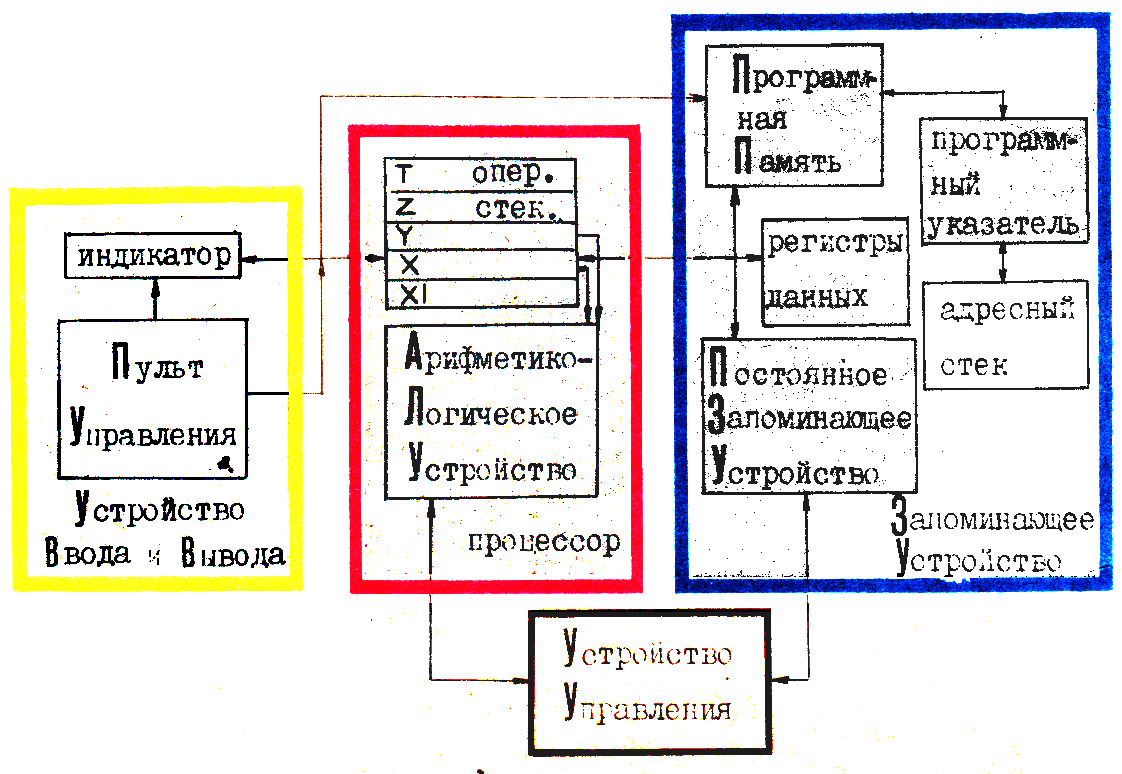
\includegraphics[width=\textwidth]{princip_scheme}

Принципиальная схема микрокаль­кулятора изображена на рисунке. Основными ее элементами являются устройство ввода и вывода информа­ции (УВВ), устройство преобразова­ния информации (процессор), запо­минающее устройство (ЗУ) и устрой­ство управления (УУ).

Устройство ввода и вывода — един­ственное, которое мы непосредствен­но видим. Состоит оно из клавиату­ры, совмещающей функции устрой­ства ввода и пульта управления, и индикатора. Программа и числа, вво­димые с клавиатуры, отображаются на индикаторе. Туда же выводятся результаты вычислений. Индикатор, вообще говоря, — единственное «ок­но» в память машины, с помощью которого можно получить сведения о ее содержимом.

Команда, введенная с клавиатуры, попадает в запоминающее устройство. Состоит ЗУ из нескольких различных секций: программная па­мять, регистры данных, постоянное запоминающее устройство (ПЗУ), а также программный указатель и ад­ресный стек.

Программная память (ПП) пред­ставляет собой набор ячеек, в каж­дую из которых можно записать один код. Всего таких ячеек 98, ну­меруются они двузначными числами  от 00 до 97. Количество ячеек опре­деляет максимальную длину програм­мы, которую можно ввести в память микрокалькулятору. Организована ПП наподобие «колеса обозрения». Адрес текущей ячейки записывается в программном указателе. При вво­де команды адрес этот автоматиче­ски увеличивается на единицу и «ко­лесо» поворачивается, подготавливая следующую «кабинку» (ячейку) для приема очередного «пассажира» (команды). Содержимое программно­го указателя можно изменять — с пульта или программным путем (об этом позже). При этом «колесо» мо­жет поворачиваться в любую сторо­ну на заданное число позиций. Ко­гда все 98 ячеек программной памя­ти заполнены, попытка ввести новую команду приводит к повороту «ко­леса» в начальное положение и команда попадает в первый адрес памяти, естественно стирая его ста­рое содержимое.

Адресный стек состоит из пяти ячеек и используется для запомина­ния адреса команды, на которую нужно передать управление после окончания работы какой-либо под­программы (об использовании под­программ будет сказано в одной из следующих статей).

Регистры данных служат для за­писи и хранения числовой информа­ции. Всего их 14. Таково максималь­ное количество чисел, которые мож­но одновременно хранить в памяти ПМК.

Постоянное запоминающее устрой­ство содержит программы, которые, собственно, и организуют процесс вычислений. Эти программы нельзя изменить, они реализованы не про­граммно, а аппаратурно, то есть представляют собой совокупность электронных схем. Их нельзя даже прочесть, к ним можно лишь обра­щаться и получать результаты их ра­боты. Именно программы из ПЗУ подсчитывают значения функций, названия которых записаны на кла­виатуре, обеспечивают выполнение арифметических операций.

Выполняет же все операции по программам, хранящимся в ПЗУ, процессор — точнее, арифметическо- логическое устройство (АЛУ), рабо­тающее совместно с операционным стеком. В этом стеке 5 регистров: XI, X, Y, Z, Т. Числа движутся по регистрам либо автоматически (при выполнении некоторых операций), либо подчиняясь специальным коман­дам. Подробно движение информа­ции в стековых регистрах будет рас­смотрено в одной из следующих ста­тей. Особо важны два регистра: X и Y. Из них АЛУ черпает число­вую информацию для выполнения двухместных операций: сложения, вы­читания, умножения, деления и воз­ведения в степень. Одноместные опе­рации: извлечение квадратного кор­ня, возведение в квадрат, вычисле­ние тригонометрических функций и т. д. — производятся над содер­жимым регистра X.

В соответствии с кодом команды АЛУ вырабатывает результат опе­рации и помещает его в регистр X. На экране отображается лишь содер­жимое этого регистра. Так что на индикаторе во время работы ПМК мелькают промежуточные результа­ты вычислений, появляющиеся в ре­гистре X.

Наконец, устройство управления обеспечивает совместную работу всех блоков ПМК.

Зная функции отдельных элемен­тов микрокалькулятора, проследим теперь полный цикл его работы при выполнении программы. Предполо­жим, что она уже введена в память, установлен режим вычислений и все необходимые числа введены в нуж­ные регистры. Нажимом клавиши «В/О» мы очищаем программный ука­затель, то есть устанавливаем его содержимое равным нулю. Клавиша, «С/П» запускает программу. Устрой­ство управления считывает команду, адрес которой записан в программ ном указателе. После ее анализа и определения типа операции команда пересылается в АЛУ. По сигналам, поступившим из УУ, процессор выра­батывает результат операции. Затем УУ опрашивает программный указа­тель и выясняет, какая команда дол­жна выполняться следующей. Потом цикл повторяется. Время выполнения цикла зависит от типа команды и колеблется от десятых долей секун­ды для команд типа записи и считы­вания, а также операций типа сло­жения, до нескольких секунд для вычисления тригонометрических функ­ций. Знание времени выполнения от­дельных команд помогает строить бо­лее быстродействующие программы.

Теперь подведем итоги.
\begin{enumerate}
\tightlist
\item Микрокалькулятор может рабо­тать в двух режимах: 1) ввода и ре­дактирования программ и 2) вычис­лений. Первый устанавливается кла­вишами «F ПРГ», второй — «F АВТ». При включении ПМК автоматически устанавливается режим вычислений.
\item Программа для микрокалькуля­тора состоит из последовательности команд, вводится с клавиатуры и записывается в программную память. Помните, что адрес, который высве­чивается при вводе в правом углу индикатора, — это адрес следующей вводимой команды.
\item Порядок работы с программой.
\begin{enumerate}[label=\arabic*)]
\item Установить режим «F ПРГ».
\item Ввести программу.
\item Перейти в режим вычисле­ний «F АВТ».
\item Ввести постоянные в адресу­емые регистры.
\item Установить начальный адрес считывания программы.
\item Набрать на клавиатуре значе­ние переменного параметра.
\item Запустить программу на счет.
\item Если нужно повторить рас­чет для другого значения пе­ременного параметра, перей­ти к пункту 6.
\end{enumerate}
\item Максимальная длина програм­мы — 98 шагов, максимальное коли­чество чисел, которые могут одно­временно храниться в памяти, — 14.
\end{enumerate}

\subparagraph{двоичная система}
10 + 10 = 100!
Это не ошибка и не опечатка. Именно такой результат получается, если числа записаны в двоичной системе счисле­ния.

Системой счисления называется способ выражения и записи чисел. Числа записываются в виде последовательности специ­альных символов. Смысл каждого символа зависит от пози­ции или разряда, в котором он записан. Количество единиц младшего разряда, объединяемого в одну единицу старшего, называется основанием системы, а символы, используемые для обозначения единиц каждого разряда, — цифрами.

Наиболее употребительна десятичная система. Мы на­столько привыкли к этой системе, что «раскрываем» любое число не задумываясь. Например, 512 = 2 + 1 * 10 + 5*102. Эта система представляется нам столь же естественной, как ребенку — родной язык. Но любая система счисления столь же естественна, как и любой язык. В вычислительной техни­ке используются двоичная, восьмеричная и шестнадцатеричная система. Двоичная — самая простая и наиболее удобная для технической реализации. Цифр в ней всего две — 0 и 1. Ко­гда в разряде (а называется двоичный разряд «бит»; несколь­ко двоичных разрядов, чаще всего восемь, объединяются в «байт» — величину, с которой ЭВМ работает как с одним целым) накапливаются две единицы, то они заменяются еди­ницей старшего разряда. Число 210 (цифрой внизу обознача­ется основание системы) в двоичной системе записывается как 102. Вообще любое число, записанное в n-ричной системе, пе­реводится в десятичную очень просто. К последней n-ричной цифре прибавляется предпоследняя, умноженная на n, затем стоящая перед ней и умноженная на n2, и т. д. Скажем, дво­ичное число 1012 = 1+0*2 + 1*22 = 510. Привлекательность двоичной системы, как уже говорилось, — в простоте техни­ческой реализации. Каждый разряд — это некоторое устрой­ство, которое может находиться всего в двух состояниях.

В микрокалькуляторе для размещения одного символа кода отводится «тетрада» — четыре двоичных разряда. Легко под­считать максимальное число, которое можно записать таким образом: 11112 - 1 + 1 • 2 + 1 • 22 + 1 • 23 = 1510. Значит, ко­ды должны изображаться числами в шестнадцатеричной си­стеме. Так как десятичных знаков для изображения таких чисел не хватает, приходится «выдумывать» дополнительные символы. В ПМК число 10 изображается символом «—», 11 — «L», 12 — «С», 13 — «Г», 14 — «Е». «Цифра» 15 в обозначе ниях кодов не используется.

\section{Язык микрокаль­кулятора}
ИГОРЬ ДАНИЛОВ,
кандидат технических наук

Язык микрокалькулятора (как и любой язык) представляет собой на­бор символов, а также правил, опре­деляющих, как с помощью этих сим­волов писать и понимать написан­ное.
Правда, в отличие, скажем, от рус­ского языка, где слова расчленяются на буквы, изменяются при склоне­нии или спряжении, язык микрокаль­кулятора напоминает скорее китай­ский либо японский. Его «словарь» состоит из несклоняемых слов-иеро­глифов, и лишь порядком их следо­вания определяется смысл текстов — программ для ПМК. Каждый из ие­роглифов — это имя команды: над­пись на клавише или над ней (а в нижнем ряду — и под клавишей). Клавиши К и F самостоятельной ро­ли не играют: по своему действию они подобны переключателю регист­ров пишущей машинки. Если требует­ся иероглиф, начертанный на клави­ше, то нужно нажать только ее, ес­ли же иероглиф, написанный над кла­вишей, то предварительно необходи­мо воспользоваться клавишей F (а в некоторых случаях — клавишей К). Каждая команда, независимо от количества нажимаемых клавиш (а оно для некоторых команд доходит до трех), отображается в памяти и на индикаторе одним двузначным шестнадцатиричным числом — кодом. Исключение составляют команды пе­реходов: после них указывается ад­рес перехода, поэтому за кодом команды обязательно следует код этого адреса.

Полный набор команд «Электрони­ки БЗ-34» приведен в таблице. Ею могут пользоваться и владельцы микрокалькуляторов «Электроника МК-54» и «Электроника МК-56» — система команд у них та же самая. Различаются лишь некоторые обозна­чения X → П вместо П, П→X вместо ИП, X ←→У вместо XY и В↑ вместо ↑, а также названия обратных тригонометрических функ­ций — $sin^{-1}$, $cos^{-1}$, $tg^{-1}$ вместо arcsin, arccos, arctg. Смысл же опе­раций и их коды полностью идентич­ные приведенным в таблице.

Условно всю совокупность команд можно разбить на два класса. К пер­вому относятся команды, используе­мые в программе; ко второму — команды, предписывающие порядок работы ПМК. Последние вводятся в режиме вычислений; мы рассмотрим их при описании процесса отладки программ.

Первый класс можно подразделить на четыре группы: 1) вычислительные команды; 2) команды обмена инфор­мацией; 3) команды управления хо­дом вычислений; 4) команды, исполь­зующие режим косвенной адресации. Последние по своим функциям не от­личаются от команд второй и треть­ей групп, но, поскольку используют иной режим адресации, будут рас­смотрены отдельно. Особняком стоит команда К НОП.

К первой группе относятся преж­де всего команды арифметических операций: сложение + (код 10), вычитание — (11), умножение X (12) и деление ÷(13). Все они дву­местные — работают с содержимым двух регистров стека X и Y, причем при вычитании в X записывается вы­читаемое, а при делении — дели­тель. Результат каждой из арифме­тических операций заносится в ре­гистр X, прежнее содержимое этого регистра перемещается в XI. То, что было в Y, пропадает, замещаясь числом из регистра Z, а в Z зано­сится содержимое регистра Т. Но при этом прежнее содержимое регистра Т остается и на своем месте.

Надо сказать, что микрокалькуля­тор способен работать не со всяки­ми числами. Максимальное не дол­жно превосходить $10^{100}$ (точнее, $9,9999999*10^{99}$), минимальное дол­жно быть не меньше $10^{99}$ — в про­тивном случае вместо нормального восьмиразрядного числа в память и на индикатор запишется «чистый» нуль. Наибольшую осторожность на­до соблюдать при умножениях и де­лениях. Иногда случается, что конеч­ный результат цепочки операций ле­жит в пределах возможностей ПМК, а на промежуточном этапе возника­ет авост. Его можно избежать, пра­вильно организуя процесс вычисле­ний.

Рассмотрим простой пример. Нуж­но вычислить значение дроби $a*b/c$, где $а=2*10^{51}$, $b=3*10^{49}$, $с=4*10^{50}$. Легко видеть, что резуль­тат ($1,5*10^{50}$) лежит в допустимых пределах. Но если соответствующий фрагмент программы записать так: ИП А, ИП В, X, ИП С, ÷, то есть сначала выполнять умножение (мы считаем, что исходные величины хра­нятся в одноименных регистрах), то после первого же действия получает­ся число $6*10^{100}$, возникает «аварий­ный» останов, на экране появляется сообщение ЕГГО.Г и вычисления прекращаются. Если же выполнять сначала деление (например, записать тот же фрагмент так: ИП А, ИП С, ÷, ИП В, X)» то никаких неприят­ностей не произойдет.

К арифметическим можно отнести и команду (—) (код 0L). Она од­номестная, использует только регистр X. При ее выполнении меняется знак числа, находящегося в этом регист­ре (плюс на минус или наоборот).

Остальные вычислительные коман­ды используются для расчета значе­ний различных функций. Их назва­ния написаны над соответствующими клавишами. Чтобы получить значе­ние какой-либо из них, нужно пред- варительно нажать клавишу F, но для краткости при описании команд мы ее упоминать не будем.

Какие же функции доступны на­шему ПМК? Вот они: извлечение квадратного корня $\sqrt{}$ (код 21);
возведение в квадрат $X^{2}$ (22); полу­чение обратной величины $1/X$ (23); возведение числа 10 в любую сте­пень $10^{x}$ (15) и возведение в степень числа е, основания натуральных логарифмов $e^{x}$ (16); вычисление де­сятичного и натурального логариф­мов lg (17) и ln (18); вычисление тригонометрических функций (аргу­менты могут быть заданы как в гра­дусах, так и в радианах) sin (1C), cos (1Г), tg (1E), а также обратных тригонометрических функций arcsin (19), arccos (1—) и arctg (1L). Ар­гумент для каждой из этих функций берется из регистра X, туда же за­писывается результат, а аргумент по­сле выполнения операции переме­щается в XI. Содержимое других ре­гистров не меняется.

\end{document}
